\documentclass[12pt,letterpaper]{article}
\usepackage[margin=0.6in, includehead, includefoot, headheight=18pt, headsep=0.22in, footskip=0.4in]{geometry}
\usepackage[T1]{fontenc}
\usepackage[scaled=0.95]{helvet}
\renewcommand{\familydefault}{\sfdefault}
\usepackage{tikz}
\usetikzlibrary{arrows.meta}
\usepackage{array}
\usepackage{enumitem}
\usepackage{fancyhdr}
\pagestyle{fancy}
\fancyhf{}
\fancyhead[L]{Week 9 / Bouncing paths / Grades 2--3}
\fancyfoot[L]{Bellingham Math Circle / Week 9 / F09-M-v4}
\fancyfoot[R]{\thepage}
\renewcommand{\headrulewidth}{0pt}
\renewcommand{\footrulewidth}{0pt}
\setlength{\parindent}{0pt}
\setlength{\parskip}{6pt}
\raggedright
\newcommand{\prob}[1]{\textbf{Problem #1:}}
\begin{document}
\noindent\begin{minipage}[c]{0.56\textwidth}\setlength{\parskip}{5pt}
The ball starts at the dot in the bottom left corner of a table and rolls up and to the right, crossing each square from corner to corner. It bounces off every wall it hits and stops when it reaches a corner of the table. Each time the ball hits a wall counts as one bounce; reaching the corner at the end does not count. A 7 by 3 table is 7 squares wide and 3 squares high.

Partners take turns: one predicts where the ball will stop, and the other traces the path.
\end{minipage}\hfill
\begin{minipage}[c]{0.4\textwidth}\centering
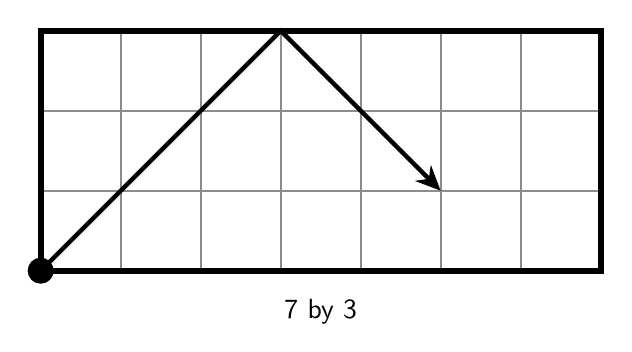
\begin{tikzpicture}[x=1in, y=1in]
\draw[black!45, line width=0.6pt] (0,0) -- (0,1.2);
\draw[black!45, line width=0.6pt] (0.4,0) -- (0.4,1.2);
\draw[black!45, line width=0.6pt] (0.8,0) -- (0.8,1.2);
\draw[black!45, line width=0.6pt] (1.2,0) -- (1.2,1.2);
\draw[black!45, line width=0.6pt] (1.6,0) -- (1.6,1.2);
\draw[black!45, line width=0.6pt] (2,0) -- (2,1.2);
\draw[black!45, line width=0.6pt] (2.4,0) -- (2.4,1.2);
\draw[black!45, line width=0.6pt] (2.8,0) -- (2.8,1.2);
\draw[black!45, line width=0.6pt] (0,0) -- (2.8,0);
\draw[black!45, line width=0.6pt] (0,0.4) -- (2.8,0.4);
\draw[black!45, line width=0.6pt] (0,0.8) -- (2.8,0.8);
\draw[black!45, line width=0.6pt] (0,1.2) -- (2.8,1.2);
\draw[line width=2.2pt] (0,0) rectangle (2.8,1.2);
\draw[line width=1.6pt, -{Stealth[length=9pt,width=8pt]}] (0,0) -- (0.4,0.4) -- (0.8,0.8) -- (1.2,1.2) -- (1.6,0.8) -- (2,0.4);
\fill (0,0) circle (0.065);
\node[anchor=north, inner sep=0pt] at (1.4,-0.14) {\normalsize 7 by 3};
\end{tikzpicture}
\end{minipage}

\vspace*{0.05in}
\prob{1} Trace the path on each table. Under each table, write the corner where the ball stops and the number of bounces.
\begin{center}
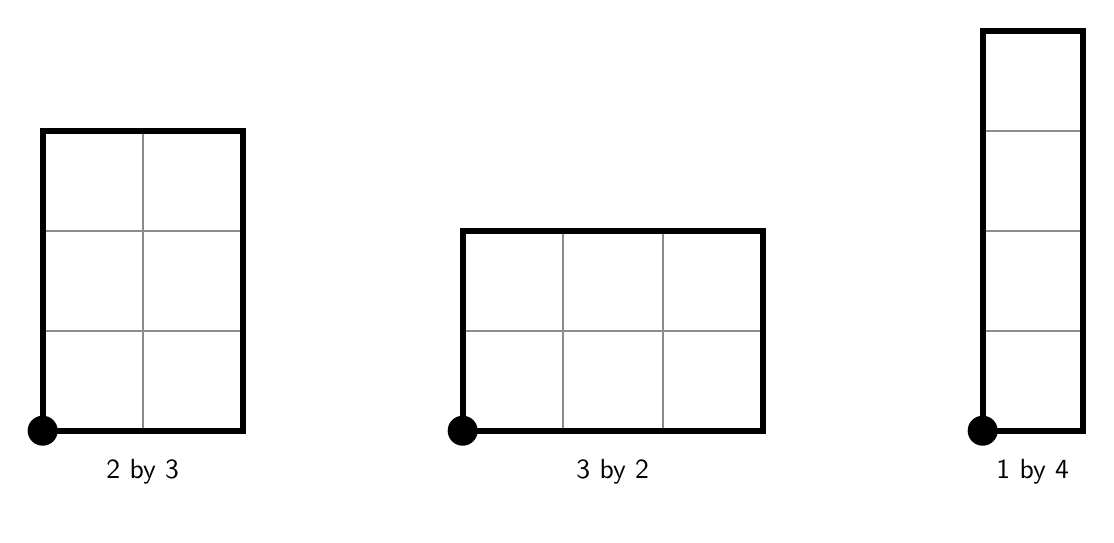
\begin{tikzpicture}[x=1in, y=1in]
\draw[black!45, line width=0.6pt] (0,0) -- (0,1.5);
\draw[black!45, line width=0.6pt] (0.5,0) -- (0.5,1.5);
\draw[black!45, line width=0.6pt] (1,0) -- (1,1.5);
\draw[black!45, line width=0.6pt] (0,0) -- (1,0);
\draw[black!45, line width=0.6pt] (0,0.5) -- (1,0.5);
\draw[black!45, line width=0.6pt] (0,1) -- (1,1);
\draw[black!45, line width=0.6pt] (0,1.5) -- (1,1.5);
\draw[line width=2.2pt] (0,0) rectangle (1,1.5);
\fill (0,0) circle (0.075);
\node[anchor=north, inner sep=0pt] at (0.5,-0.14) {\normalsize 2 by 3};
\draw[black!45, line width=0.6pt] (2.1,0) -- (2.1,1);
\draw[black!45, line width=0.6pt] (2.6,0) -- (2.6,1);
\draw[black!45, line width=0.6pt] (3.1,0) -- (3.1,1);
\draw[black!45, line width=0.6pt] (3.6,0) -- (3.6,1);
\draw[black!45, line width=0.6pt] (2.1,0) -- (3.6,0);
\draw[black!45, line width=0.6pt] (2.1,0.5) -- (3.6,0.5);
\draw[black!45, line width=0.6pt] (2.1,1) -- (3.6,1);
\draw[line width=2.2pt] (2.1,0) rectangle (3.6,1);
\fill (2.1,0) circle (0.075);
\node[anchor=north, inner sep=0pt] at (2.85,-0.14) {\normalsize 3 by 2};
\draw[black!45, line width=0.6pt] (4.7,0) -- (4.7,2);
\draw[black!45, line width=0.6pt] (5.2,0) -- (5.2,2);
\draw[black!45, line width=0.6pt] (4.7,0) -- (5.2,0);
\draw[black!45, line width=0.6pt] (4.7,0.5) -- (5.2,0.5);
\draw[black!45, line width=0.6pt] (4.7,1) -- (5.2,1);
\draw[black!45, line width=0.6pt] (4.7,1.5) -- (5.2,1.5);
\draw[black!45, line width=0.6pt] (4.7,2) -- (5.2,2);
\draw[line width=2.2pt] (4.7,0) rectangle (5.2,2);
\fill (4.7,0) circle (0.075);
\node[anchor=north, inner sep=0pt] at (4.95,-0.14) {\normalsize 1 by 4};
\path (0,-0.42) rectangle (5.2,2);
\end{tikzpicture}
\end{center}
\vspace*{0.45in}
\begin{center}
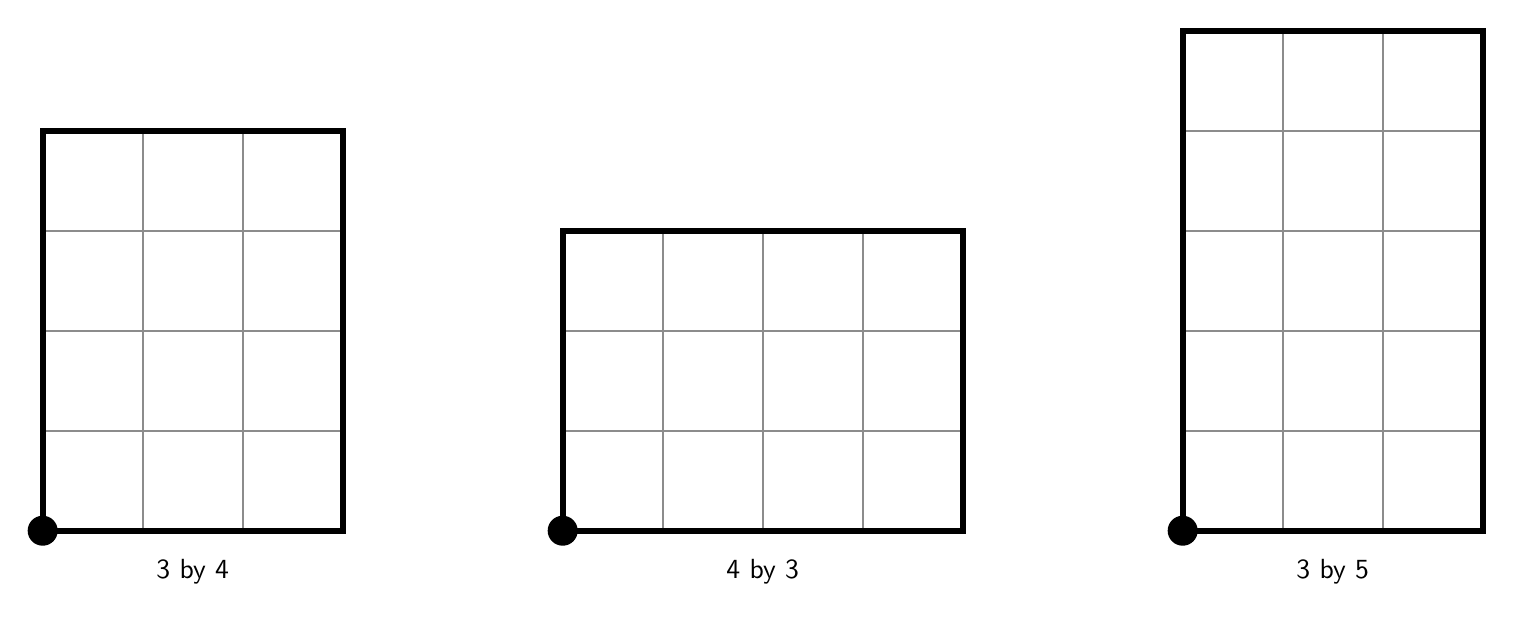
\begin{tikzpicture}[x=1in, y=1in]
\draw[black!45, line width=0.6pt] (0,0) -- (0,2);
\draw[black!45, line width=0.6pt] (0.5,0) -- (0.5,2);
\draw[black!45, line width=0.6pt] (1,0) -- (1,2);
\draw[black!45, line width=0.6pt] (1.5,0) -- (1.5,2);
\draw[black!45, line width=0.6pt] (0,0) -- (1.5,0);
\draw[black!45, line width=0.6pt] (0,0.5) -- (1.5,0.5);
\draw[black!45, line width=0.6pt] (0,1) -- (1.5,1);
\draw[black!45, line width=0.6pt] (0,1.5) -- (1.5,1.5);
\draw[black!45, line width=0.6pt] (0,2) -- (1.5,2);
\draw[line width=2.2pt] (0,0) rectangle (1.5,2);
\fill (0,0) circle (0.075);
\node[anchor=north, inner sep=0pt] at (0.75,-0.14) {\normalsize 3 by 4};
\draw[black!45, line width=0.6pt] (2.6,0) -- (2.6,1.5);
\draw[black!45, line width=0.6pt] (3.1,0) -- (3.1,1.5);
\draw[black!45, line width=0.6pt] (3.6,0) -- (3.6,1.5);
\draw[black!45, line width=0.6pt] (4.1,0) -- (4.1,1.5);
\draw[black!45, line width=0.6pt] (4.6,0) -- (4.6,1.5);
\draw[black!45, line width=0.6pt] (2.6,0) -- (4.6,0);
\draw[black!45, line width=0.6pt] (2.6,0.5) -- (4.6,0.5);
\draw[black!45, line width=0.6pt] (2.6,1) -- (4.6,1);
\draw[black!45, line width=0.6pt] (2.6,1.5) -- (4.6,1.5);
\draw[line width=2.2pt] (2.6,0) rectangle (4.6,1.5);
\fill (2.6,0) circle (0.075);
\node[anchor=north, inner sep=0pt] at (3.6,-0.14) {\normalsize 4 by 3};
\draw[black!45, line width=0.6pt] (5.7,0) -- (5.7,2.5);
\draw[black!45, line width=0.6pt] (6.2,0) -- (6.2,2.5);
\draw[black!45, line width=0.6pt] (6.7,0) -- (6.7,2.5);
\draw[black!45, line width=0.6pt] (7.2,0) -- (7.2,2.5);
\draw[black!45, line width=0.6pt] (5.7,0) -- (7.2,0);
\draw[black!45, line width=0.6pt] (5.7,0.5) -- (7.2,0.5);
\draw[black!45, line width=0.6pt] (5.7,1) -- (7.2,1);
\draw[black!45, line width=0.6pt] (5.7,1.5) -- (7.2,1.5);
\draw[black!45, line width=0.6pt] (5.7,2) -- (7.2,2);
\draw[black!45, line width=0.6pt] (5.7,2.5) -- (7.2,2.5);
\draw[line width=2.2pt] (5.7,0) rectangle (7.2,2.5);
\fill (5.7,0) circle (0.075);
\node[anchor=north, inner sep=0pt] at (6.45,-0.14) {\normalsize 3 by 5};
\path (0,-0.42) rectangle (7.2,2.5);
\end{tikzpicture}
\end{center}
\newpage
\prob{2} Trace the path on each table, and write the corner where the ball stops and the number of bounces.
\vspace*{0.1in}
\begin{center}
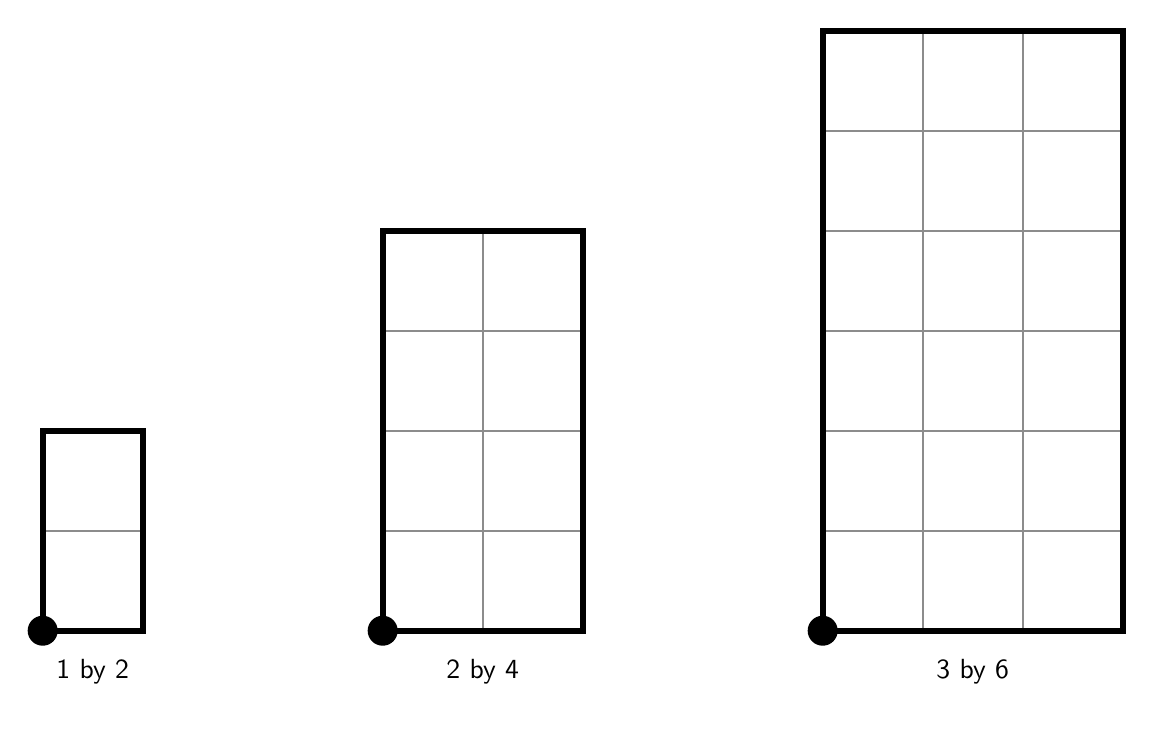
\begin{tikzpicture}[x=1in, y=1in]
\draw[black!45, line width=0.6pt] (0,0) -- (0,1);
\draw[black!45, line width=0.6pt] (0.5,0) -- (0.5,1);
\draw[black!45, line width=0.6pt] (0,0) -- (0.5,0);
\draw[black!45, line width=0.6pt] (0,0.5) -- (0.5,0.5);
\draw[black!45, line width=0.6pt] (0,1) -- (0.5,1);
\draw[line width=2.2pt] (0,0) rectangle (0.5,1);
\fill (0,0) circle (0.075);
\node[anchor=north, inner sep=0pt] at (0.25,-0.14) {\normalsize 1 by 2};
\draw[black!45, line width=0.6pt] (1.7,0) -- (1.7,2);
\draw[black!45, line width=0.6pt] (2.2,0) -- (2.2,2);
\draw[black!45, line width=0.6pt] (2.7,0) -- (2.7,2);
\draw[black!45, line width=0.6pt] (1.7,0) -- (2.7,0);
\draw[black!45, line width=0.6pt] (1.7,0.5) -- (2.7,0.5);
\draw[black!45, line width=0.6pt] (1.7,1) -- (2.7,1);
\draw[black!45, line width=0.6pt] (1.7,1.5) -- (2.7,1.5);
\draw[black!45, line width=0.6pt] (1.7,2) -- (2.7,2);
\draw[line width=2.2pt] (1.7,0) rectangle (2.7,2);
\fill (1.7,0) circle (0.075);
\node[anchor=north, inner sep=0pt] at (2.2,-0.14) {\normalsize 2 by 4};
\draw[black!45, line width=0.6pt] (3.9,0) -- (3.9,3);
\draw[black!45, line width=0.6pt] (4.4,0) -- (4.4,3);
\draw[black!45, line width=0.6pt] (4.9,0) -- (4.9,3);
\draw[black!45, line width=0.6pt] (5.4,0) -- (5.4,3);
\draw[black!45, line width=0.6pt] (3.9,0) -- (5.4,0);
\draw[black!45, line width=0.6pt] (3.9,0.5) -- (5.4,0.5);
\draw[black!45, line width=0.6pt] (3.9,1) -- (5.4,1);
\draw[black!45, line width=0.6pt] (3.9,1.5) -- (5.4,1.5);
\draw[black!45, line width=0.6pt] (3.9,2) -- (5.4,2);
\draw[black!45, line width=0.6pt] (3.9,2.5) -- (5.4,2.5);
\draw[black!45, line width=0.6pt] (3.9,3) -- (5.4,3);
\draw[line width=2.2pt] (3.9,0) rectangle (5.4,3);
\fill (3.9,0) circle (0.075);
\node[anchor=north, inner sep=0pt] at (4.65,-0.14) {\normalsize 3 by 6};
\path (0,-0.42) rectangle (5.4,3);
\end{tikzpicture}
\end{center}
\vspace*{0.5in}
\begin{center}
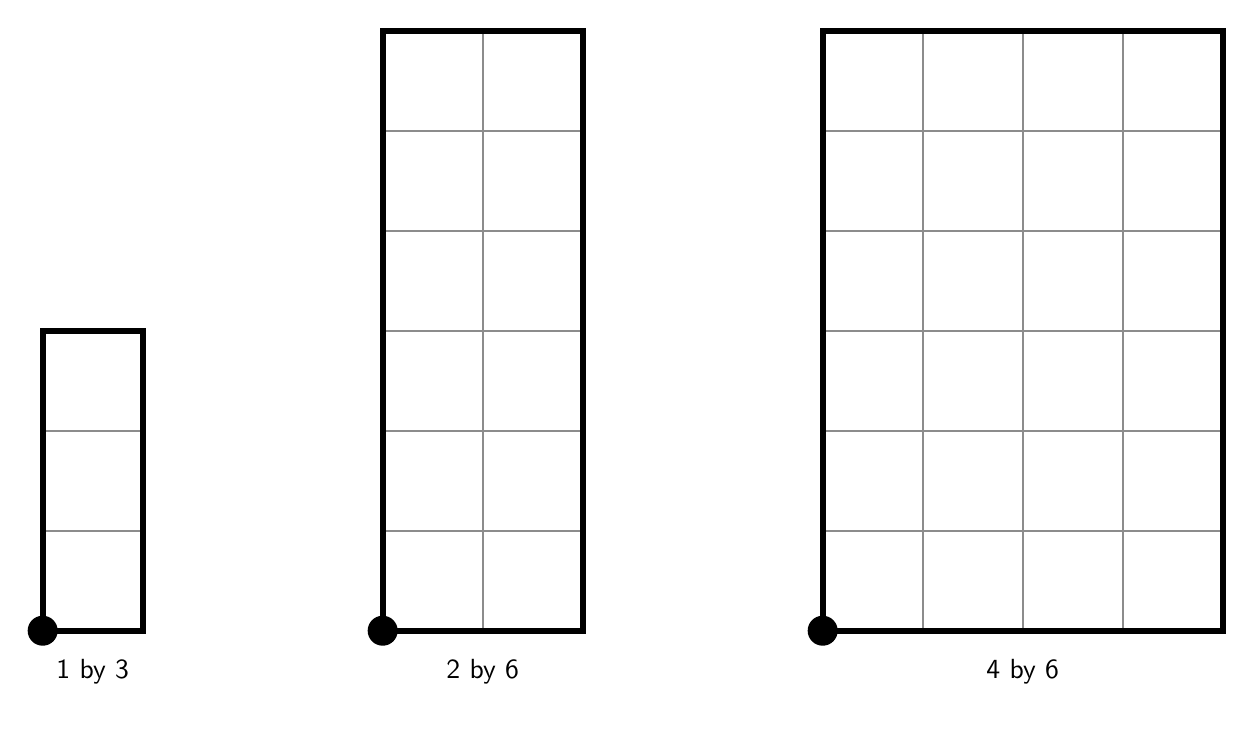
\begin{tikzpicture}[x=1in, y=1in]
\draw[black!45, line width=0.6pt] (0,0) -- (0,1.5);
\draw[black!45, line width=0.6pt] (0.5,0) -- (0.5,1.5);
\draw[black!45, line width=0.6pt] (0,0) -- (0.5,0);
\draw[black!45, line width=0.6pt] (0,0.5) -- (0.5,0.5);
\draw[black!45, line width=0.6pt] (0,1) -- (0.5,1);
\draw[black!45, line width=0.6pt] (0,1.5) -- (0.5,1.5);
\draw[line width=2.2pt] (0,0) rectangle (0.5,1.5);
\fill (0,0) circle (0.075);
\node[anchor=north, inner sep=0pt] at (0.25,-0.14) {\normalsize 1 by 3};
\draw[black!45, line width=0.6pt] (1.7,0) -- (1.7,3);
\draw[black!45, line width=0.6pt] (2.2,0) -- (2.2,3);
\draw[black!45, line width=0.6pt] (2.7,0) -- (2.7,3);
\draw[black!45, line width=0.6pt] (1.7,0) -- (2.7,0);
\draw[black!45, line width=0.6pt] (1.7,0.5) -- (2.7,0.5);
\draw[black!45, line width=0.6pt] (1.7,1) -- (2.7,1);
\draw[black!45, line width=0.6pt] (1.7,1.5) -- (2.7,1.5);
\draw[black!45, line width=0.6pt] (1.7,2) -- (2.7,2);
\draw[black!45, line width=0.6pt] (1.7,2.5) -- (2.7,2.5);
\draw[black!45, line width=0.6pt] (1.7,3) -- (2.7,3);
\draw[line width=2.2pt] (1.7,0) rectangle (2.7,3);
\fill (1.7,0) circle (0.075);
\node[anchor=north, inner sep=0pt] at (2.2,-0.14) {\normalsize 2 by 6};
\draw[black!45, line width=0.6pt] (3.9,0) -- (3.9,3);
\draw[black!45, line width=0.6pt] (4.4,0) -- (4.4,3);
\draw[black!45, line width=0.6pt] (4.9,0) -- (4.9,3);
\draw[black!45, line width=0.6pt] (5.4,0) -- (5.4,3);
\draw[black!45, line width=0.6pt] (5.9,0) -- (5.9,3);
\draw[black!45, line width=0.6pt] (3.9,0) -- (5.9,0);
\draw[black!45, line width=0.6pt] (3.9,0.5) -- (5.9,0.5);
\draw[black!45, line width=0.6pt] (3.9,1) -- (5.9,1);
\draw[black!45, line width=0.6pt] (3.9,1.5) -- (5.9,1.5);
\draw[black!45, line width=0.6pt] (3.9,2) -- (5.9,2);
\draw[black!45, line width=0.6pt] (3.9,2.5) -- (5.9,2.5);
\draw[black!45, line width=0.6pt] (3.9,3) -- (5.9,3);
\draw[line width=2.2pt] (3.9,0) rectangle (5.9,3);
\fill (3.9,0) circle (0.075);
\node[anchor=north, inner sep=0pt] at (4.9,-0.14) {\normalsize 4 by 6};
\path (0,-0.42) rectangle (5.9,3);
\end{tikzpicture}
\end{center}
\newpage
\prob{3} Before you trace these two tables, write the corner where you think the ball will stop and the number of bounces you expect. Then trace the paths to check.
\vspace*{0.1in}
\begin{center}
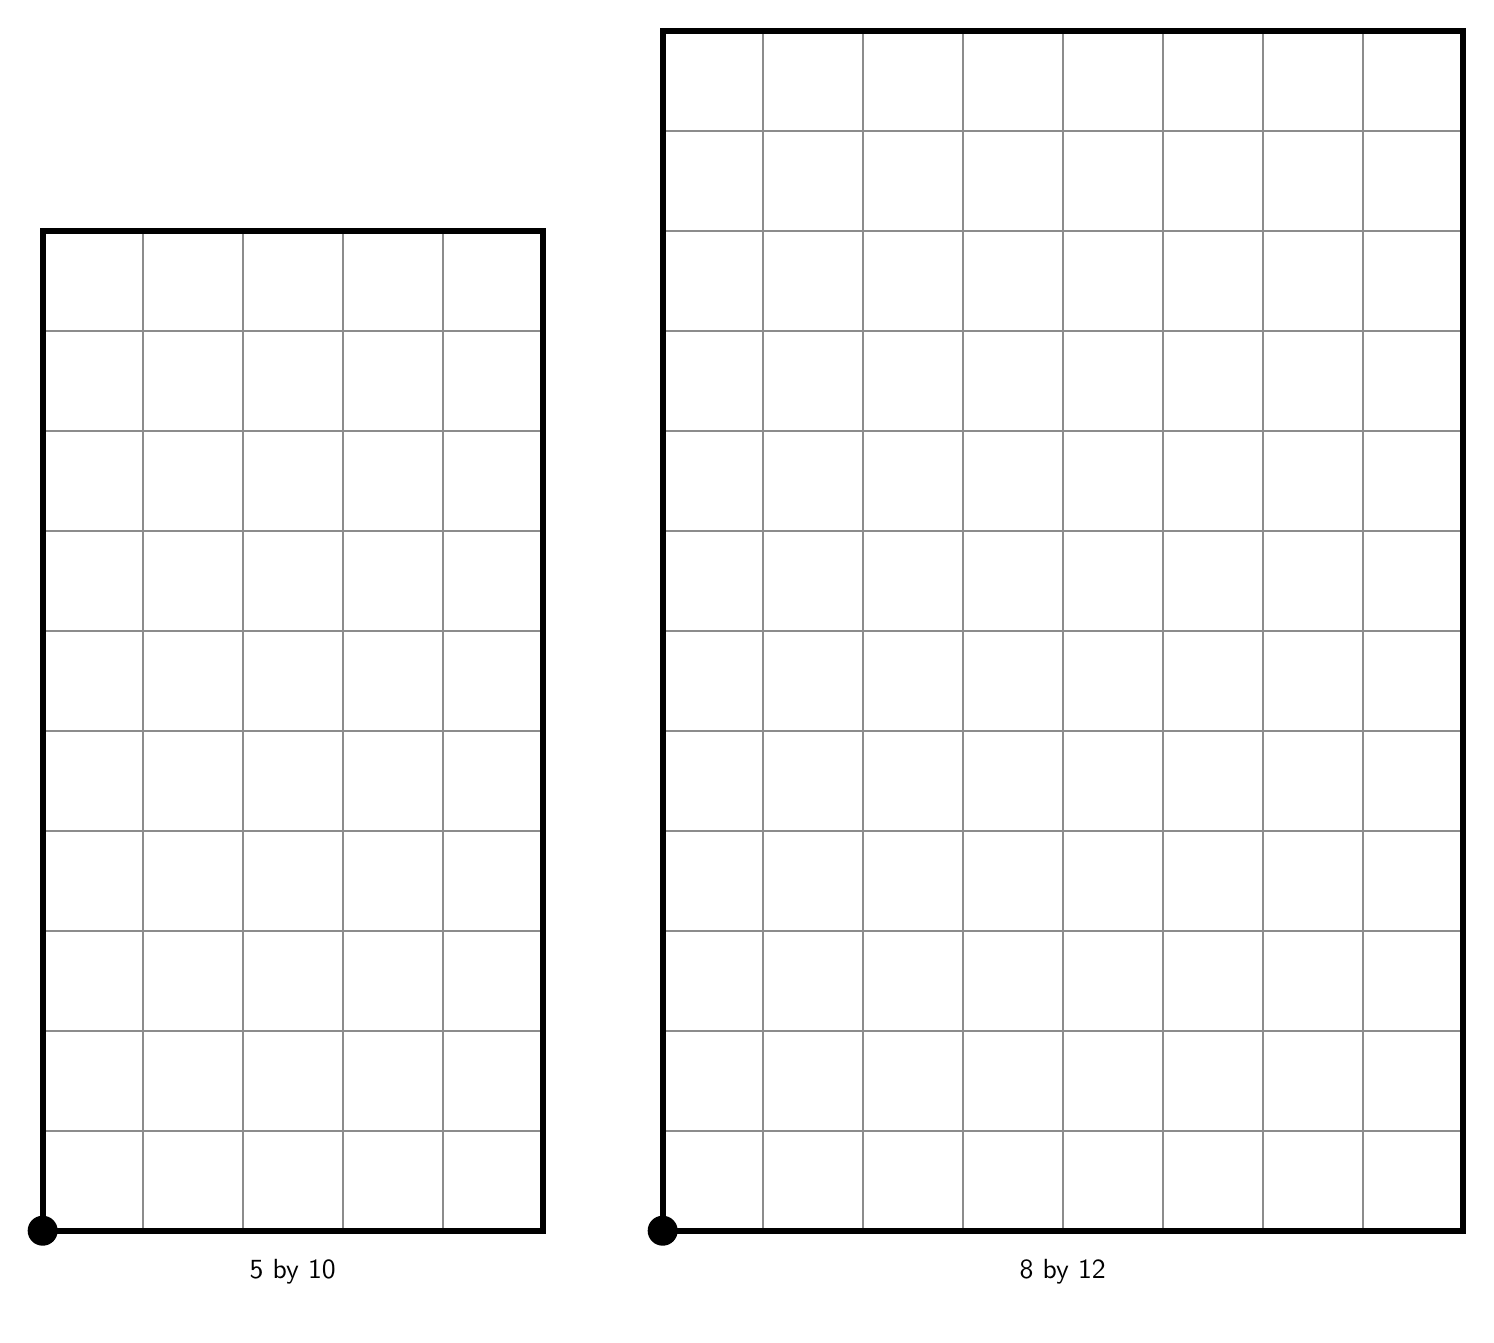
\begin{tikzpicture}[x=1in, y=1in]
\draw[black!45, line width=0.6pt] (0,0) -- (0,5);
\draw[black!45, line width=0.6pt] (0.5,0) -- (0.5,5);
\draw[black!45, line width=0.6pt] (1,0) -- (1,5);
\draw[black!45, line width=0.6pt] (1.5,0) -- (1.5,5);
\draw[black!45, line width=0.6pt] (2,0) -- (2,5);
\draw[black!45, line width=0.6pt] (2.5,0) -- (2.5,5);
\draw[black!45, line width=0.6pt] (0,0) -- (2.5,0);
\draw[black!45, line width=0.6pt] (0,0.5) -- (2.5,0.5);
\draw[black!45, line width=0.6pt] (0,1) -- (2.5,1);
\draw[black!45, line width=0.6pt] (0,1.5) -- (2.5,1.5);
\draw[black!45, line width=0.6pt] (0,2) -- (2.5,2);
\draw[black!45, line width=0.6pt] (0,2.5) -- (2.5,2.5);
\draw[black!45, line width=0.6pt] (0,3) -- (2.5,3);
\draw[black!45, line width=0.6pt] (0,3.5) -- (2.5,3.5);
\draw[black!45, line width=0.6pt] (0,4) -- (2.5,4);
\draw[black!45, line width=0.6pt] (0,4.5) -- (2.5,4.5);
\draw[black!45, line width=0.6pt] (0,5) -- (2.5,5);
\draw[line width=2.2pt] (0,0) rectangle (2.5,5);
\fill (0,0) circle (0.075);
\node[anchor=north, inner sep=0pt] at (1.25,-0.14) {\normalsize 5 by 10};
\draw[black!45, line width=0.6pt] (3.1,0) -- (3.1,6);
\draw[black!45, line width=0.6pt] (3.6,0) -- (3.6,6);
\draw[black!45, line width=0.6pt] (4.1,0) -- (4.1,6);
\draw[black!45, line width=0.6pt] (4.6,0) -- (4.6,6);
\draw[black!45, line width=0.6pt] (5.1,0) -- (5.1,6);
\draw[black!45, line width=0.6pt] (5.6,0) -- (5.6,6);
\draw[black!45, line width=0.6pt] (6.1,0) -- (6.1,6);
\draw[black!45, line width=0.6pt] (6.6,0) -- (6.6,6);
\draw[black!45, line width=0.6pt] (7.1,0) -- (7.1,6);
\draw[black!45, line width=0.6pt] (3.1,0) -- (7.1,0);
\draw[black!45, line width=0.6pt] (3.1,0.5) -- (7.1,0.5);
\draw[black!45, line width=0.6pt] (3.1,1) -- (7.1,1);
\draw[black!45, line width=0.6pt] (3.1,1.5) -- (7.1,1.5);
\draw[black!45, line width=0.6pt] (3.1,2) -- (7.1,2);
\draw[black!45, line width=0.6pt] (3.1,2.5) -- (7.1,2.5);
\draw[black!45, line width=0.6pt] (3.1,3) -- (7.1,3);
\draw[black!45, line width=0.6pt] (3.1,3.5) -- (7.1,3.5);
\draw[black!45, line width=0.6pt] (3.1,4) -- (7.1,4);
\draw[black!45, line width=0.6pt] (3.1,4.5) -- (7.1,4.5);
\draw[black!45, line width=0.6pt] (3.1,5) -- (7.1,5);
\draw[black!45, line width=0.6pt] (3.1,5.5) -- (7.1,5.5);
\draw[black!45, line width=0.6pt] (3.1,6) -- (7.1,6);
\draw[line width=2.2pt] (3.1,0) rectangle (7.1,6);
\fill (3.1,0) circle (0.075);
\node[anchor=north, inner sep=0pt] at (5.1,-0.14) {\normalsize 8 by 12};
\path (0,-0.42) rectangle (7.1,6);
\end{tikzpicture}
\end{center}
\newpage
\prob{4} On each grid, draw a table with its bottom left corner at the dot, so that the ball does what is written under the grid. If there is no such table, explain why.
\vspace*{0.1in}
\begin{center}
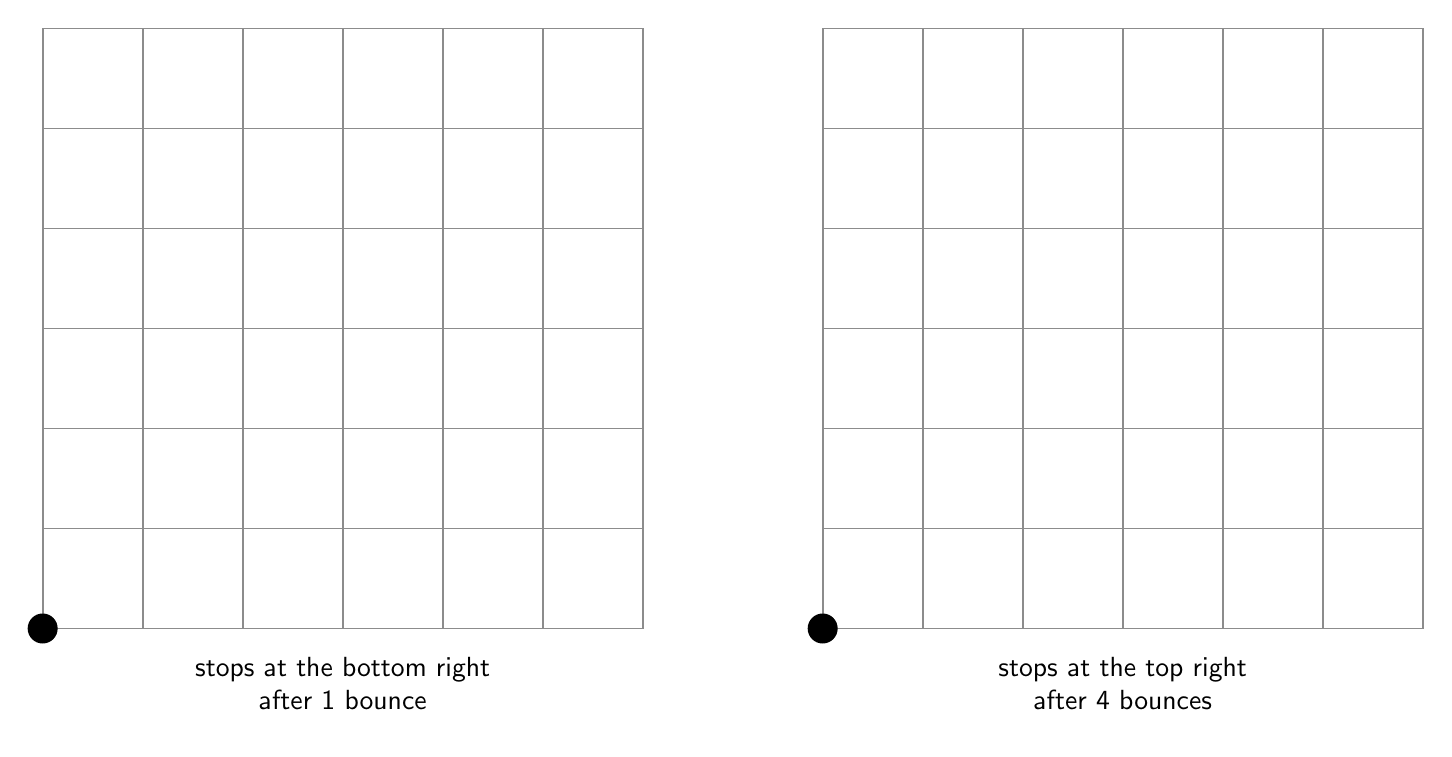
\begin{tikzpicture}[x=1in, y=1in]
\draw[black!45, line width=0.6pt] (0,0) -- (0,3);
\draw[black!45, line width=0.6pt] (0.5,0) -- (0.5,3);
\draw[black!45, line width=0.6pt] (1,0) -- (1,3);
\draw[black!45, line width=0.6pt] (1.5,0) -- (1.5,3);
\draw[black!45, line width=0.6pt] (2,0) -- (2,3);
\draw[black!45, line width=0.6pt] (2.5,0) -- (2.5,3);
\draw[black!45, line width=0.6pt] (3,0) -- (3,3);
\draw[black!45, line width=0.6pt] (0,0) -- (3,0);
\draw[black!45, line width=0.6pt] (0,0.5) -- (3,0.5);
\draw[black!45, line width=0.6pt] (0,1) -- (3,1);
\draw[black!45, line width=0.6pt] (0,1.5) -- (3,1.5);
\draw[black!45, line width=0.6pt] (0,2) -- (3,2);
\draw[black!45, line width=0.6pt] (0,2.5) -- (3,2.5);
\draw[black!45, line width=0.6pt] (0,3) -- (3,3);
\fill (0,0) circle (0.075);
\node[anchor=north, inner sep=0pt, align=center] at (1.5,-0.14) {\normalsize stops at the bottom right\\after 1 bounce};
\draw[black!45, line width=0.6pt] (3.9,0) -- (3.9,3);
\draw[black!45, line width=0.6pt] (4.4,0) -- (4.4,3);
\draw[black!45, line width=0.6pt] (4.9,0) -- (4.9,3);
\draw[black!45, line width=0.6pt] (5.4,0) -- (5.4,3);
\draw[black!45, line width=0.6pt] (5.9,0) -- (5.9,3);
\draw[black!45, line width=0.6pt] (6.4,0) -- (6.4,3);
\draw[black!45, line width=0.6pt] (6.9,0) -- (6.9,3);
\draw[black!45, line width=0.6pt] (3.9,0) -- (6.9,0);
\draw[black!45, line width=0.6pt] (3.9,0.5) -- (6.9,0.5);
\draw[black!45, line width=0.6pt] (3.9,1) -- (6.9,1);
\draw[black!45, line width=0.6pt] (3.9,1.5) -- (6.9,1.5);
\draw[black!45, line width=0.6pt] (3.9,2) -- (6.9,2);
\draw[black!45, line width=0.6pt] (3.9,2.5) -- (6.9,2.5);
\draw[black!45, line width=0.6pt] (3.9,3) -- (6.9,3);
\fill (3.9,0) circle (0.075);
\node[anchor=north, inner sep=0pt, align=center] at (5.4,-0.14) {\normalsize stops at the top right\\after 4 bounces};
\path (0,-0.5) rectangle (6.9,3);
\end{tikzpicture}
\end{center}
\vspace*{0.35in}
\begin{center}
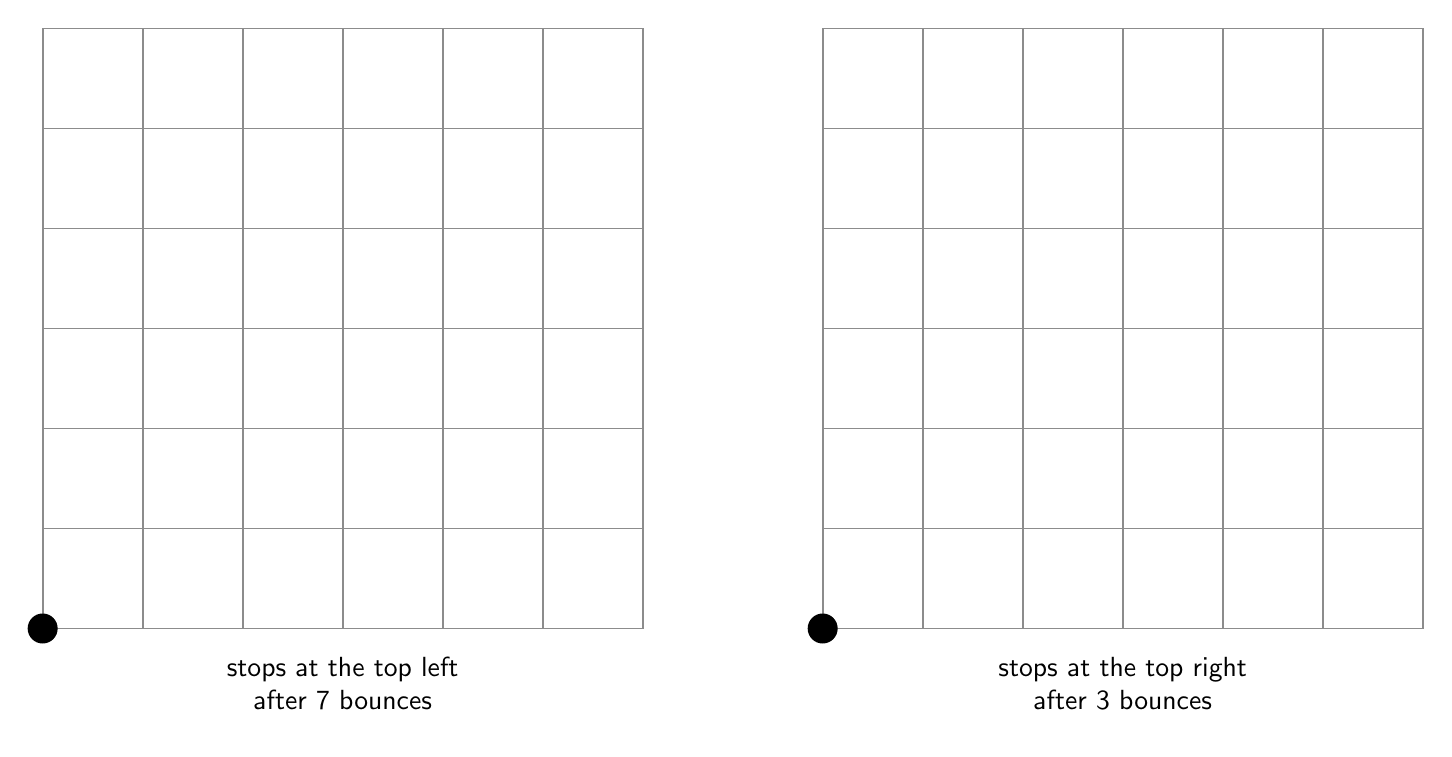
\begin{tikzpicture}[x=1in, y=1in]
\draw[black!45, line width=0.6pt] (0,0) -- (0,3);
\draw[black!45, line width=0.6pt] (0.5,0) -- (0.5,3);
\draw[black!45, line width=0.6pt] (1,0) -- (1,3);
\draw[black!45, line width=0.6pt] (1.5,0) -- (1.5,3);
\draw[black!45, line width=0.6pt] (2,0) -- (2,3);
\draw[black!45, line width=0.6pt] (2.5,0) -- (2.5,3);
\draw[black!45, line width=0.6pt] (3,0) -- (3,3);
\draw[black!45, line width=0.6pt] (0,0) -- (3,0);
\draw[black!45, line width=0.6pt] (0,0.5) -- (3,0.5);
\draw[black!45, line width=0.6pt] (0,1) -- (3,1);
\draw[black!45, line width=0.6pt] (0,1.5) -- (3,1.5);
\draw[black!45, line width=0.6pt] (0,2) -- (3,2);
\draw[black!45, line width=0.6pt] (0,2.5) -- (3,2.5);
\draw[black!45, line width=0.6pt] (0,3) -- (3,3);
\fill (0,0) circle (0.075);
\node[anchor=north, inner sep=0pt, align=center] at (1.5,-0.14) {\normalsize stops at the top left\\after 7 bounces};
\draw[black!45, line width=0.6pt] (3.9,0) -- (3.9,3);
\draw[black!45, line width=0.6pt] (4.4,0) -- (4.4,3);
\draw[black!45, line width=0.6pt] (4.9,0) -- (4.9,3);
\draw[black!45, line width=0.6pt] (5.4,0) -- (5.4,3);
\draw[black!45, line width=0.6pt] (5.9,0) -- (5.9,3);
\draw[black!45, line width=0.6pt] (6.4,0) -- (6.4,3);
\draw[black!45, line width=0.6pt] (6.9,0) -- (6.9,3);
\draw[black!45, line width=0.6pt] (3.9,0) -- (6.9,0);
\draw[black!45, line width=0.6pt] (3.9,0.5) -- (6.9,0.5);
\draw[black!45, line width=0.6pt] (3.9,1) -- (6.9,1);
\draw[black!45, line width=0.6pt] (3.9,1.5) -- (6.9,1.5);
\draw[black!45, line width=0.6pt] (3.9,2) -- (6.9,2);
\draw[black!45, line width=0.6pt] (3.9,2.5) -- (6.9,2.5);
\draw[black!45, line width=0.6pt] (3.9,3) -- (6.9,3);
\fill (3.9,0) circle (0.075);
\node[anchor=north, inner sep=0pt, align=center] at (5.4,-0.14) {\normalsize stops at the top right\\after 3 bounces};
\path (0,-0.5) rectangle (6.9,3);
\end{tikzpicture}
\end{center}
\newpage
\prob{5} Play this game with your partner. One player draws a table on the grid, no more than 6 squares wide and 6 squares high, and marks its dot. The other player says where the ball will stop and how many times it will bounce, and then traces the path. The player who predicted scores 1 point for the right corner and 1 point for the right number of bounces. Then swap jobs. After each player has predicted three tables, the player with more points wins.
\vspace*{0.05in}
\begin{center}
\begin{tikzpicture}[x=1in, y=1in]
\draw[black!45, line width=0.6pt] (0,0) -- (0,7.5);
\draw[black!45, line width=0.6pt] (0.5,0) -- (0.5,7.5);
\draw[black!45, line width=0.6pt] (1,0) -- (1,7.5);
\draw[black!45, line width=0.6pt] (1.5,0) -- (1.5,7.5);
\draw[black!45, line width=0.6pt] (2,0) -- (2,7.5);
\draw[black!45, line width=0.6pt] (2.5,0) -- (2.5,7.5);
\draw[black!45, line width=0.6pt] (3,0) -- (3,7.5);
\draw[black!45, line width=0.6pt] (3.5,0) -- (3.5,7.5);
\draw[black!45, line width=0.6pt] (4,0) -- (4,7.5);
\draw[black!45, line width=0.6pt] (4.5,0) -- (4.5,7.5);
\draw[black!45, line width=0.6pt] (5,0) -- (5,7.5);
\draw[black!45, line width=0.6pt] (5.5,0) -- (5.5,7.5);
\draw[black!45, line width=0.6pt] (6,0) -- (6,7.5);
\draw[black!45, line width=0.6pt] (6.5,0) -- (6.5,7.5);
\draw[black!45, line width=0.6pt] (7,0) -- (7,7.5);
\draw[black!45, line width=0.6pt] (0,0) -- (7,0);
\draw[black!45, line width=0.6pt] (0,0.5) -- (7,0.5);
\draw[black!45, line width=0.6pt] (0,1) -- (7,1);
\draw[black!45, line width=0.6pt] (0,1.5) -- (7,1.5);
\draw[black!45, line width=0.6pt] (0,2) -- (7,2);
\draw[black!45, line width=0.6pt] (0,2.5) -- (7,2.5);
\draw[black!45, line width=0.6pt] (0,3) -- (7,3);
\draw[black!45, line width=0.6pt] (0,3.5) -- (7,3.5);
\draw[black!45, line width=0.6pt] (0,4) -- (7,4);
\draw[black!45, line width=0.6pt] (0,4.5) -- (7,4.5);
\draw[black!45, line width=0.6pt] (0,5) -- (7,5);
\draw[black!45, line width=0.6pt] (0,5.5) -- (7,5.5);
\draw[black!45, line width=0.6pt] (0,6) -- (7,6);
\draw[black!45, line width=0.6pt] (0,6.5) -- (7,6.5);
\draw[black!45, line width=0.6pt] (0,7) -- (7,7);
\draw[black!45, line width=0.6pt] (0,7.5) -- (7,7.5);
\path (0,-0) rectangle (7,7.5);
\end{tikzpicture}
\end{center}
\newpage
\prob{6} Find every table no more than 6 squares wide and no more than 6 squares high where the ball bounces exactly once. Explain how you know you have found them all.
\vspace*{0.05in}
\begin{center}
\begin{tikzpicture}[x=1in, y=1in]
\draw[black!45, line width=0.6pt] (0,0) -- (0,5);
\draw[black!45, line width=0.6pt] (0.5,0) -- (0.5,5);
\draw[black!45, line width=0.6pt] (1,0) -- (1,5);
\draw[black!45, line width=0.6pt] (1.5,0) -- (1.5,5);
\draw[black!45, line width=0.6pt] (2,0) -- (2,5);
\draw[black!45, line width=0.6pt] (2.5,0) -- (2.5,5);
\draw[black!45, line width=0.6pt] (3,0) -- (3,5);
\draw[black!45, line width=0.6pt] (3.5,0) -- (3.5,5);
\draw[black!45, line width=0.6pt] (4,0) -- (4,5);
\draw[black!45, line width=0.6pt] (4.5,0) -- (4.5,5);
\draw[black!45, line width=0.6pt] (5,0) -- (5,5);
\draw[black!45, line width=0.6pt] (5.5,0) -- (5.5,5);
\draw[black!45, line width=0.6pt] (6,0) -- (6,5);
\draw[black!45, line width=0.6pt] (6.5,0) -- (6.5,5);
\draw[black!45, line width=0.6pt] (7,0) -- (7,5);
\draw[black!45, line width=0.6pt] (0,0) -- (7,0);
\draw[black!45, line width=0.6pt] (0,0.5) -- (7,0.5);
\draw[black!45, line width=0.6pt] (0,1) -- (7,1);
\draw[black!45, line width=0.6pt] (0,1.5) -- (7,1.5);
\draw[black!45, line width=0.6pt] (0,2) -- (7,2);
\draw[black!45, line width=0.6pt] (0,2.5) -- (7,2.5);
\draw[black!45, line width=0.6pt] (0,3) -- (7,3);
\draw[black!45, line width=0.6pt] (0,3.5) -- (7,3.5);
\draw[black!45, line width=0.6pt] (0,4) -- (7,4);
\draw[black!45, line width=0.6pt] (0,4.5) -- (7,4.5);
\draw[black!45, line width=0.6pt] (0,5) -- (7,5);
\path (0,-0) rectangle (7,5);
\end{tikzpicture}
\end{center}
\newpage
\prob{7} With a ruler and a dark marker, draw a straight line from the dot to the opposite corner of each sheet. How many thick lines inside the sheet does each line cross? Then cut out the tables each line passes through, keeping them in one piece. Fold them on the thick lines until they are the size of one table with the dot in front. Hold them up to the light, and copy the path you see onto the small table beside the sheet.
\vspace*{0.1in}
\begin{center}
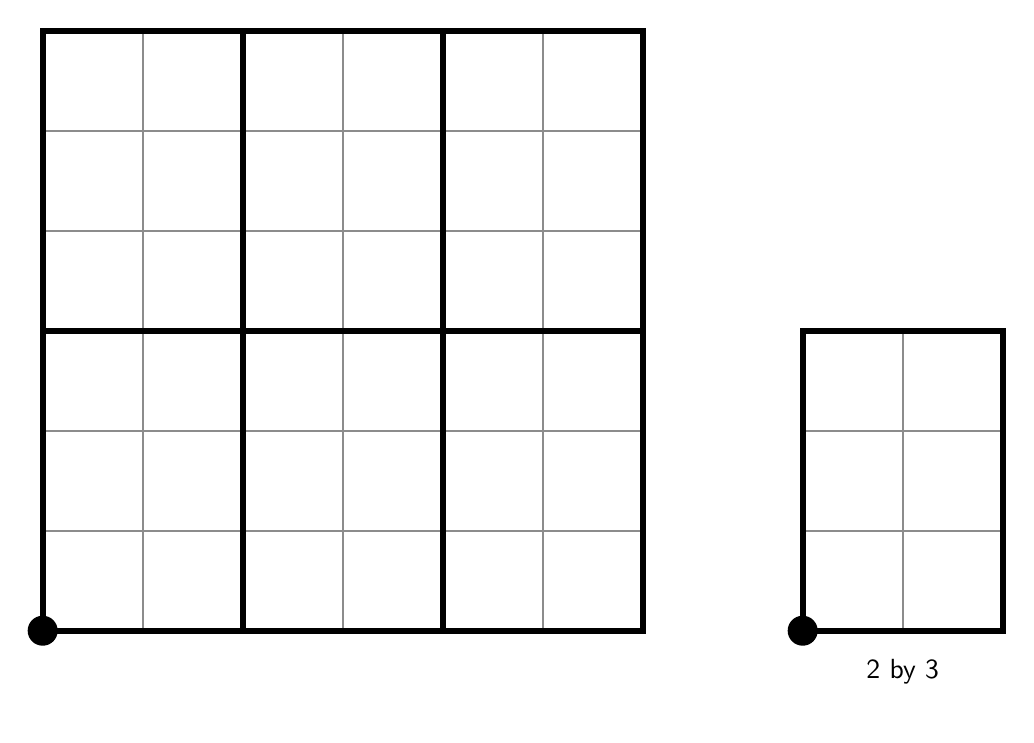
\begin{tikzpicture}[x=1in, y=1in]
\draw[black!45, line width=0.6pt] (0,0) -- (0,3);
\draw[black!45, line width=0.6pt] (0.5,0) -- (0.5,3);
\draw[black!45, line width=0.6pt] (1,0) -- (1,3);
\draw[black!45, line width=0.6pt] (1.5,0) -- (1.5,3);
\draw[black!45, line width=0.6pt] (2,0) -- (2,3);
\draw[black!45, line width=0.6pt] (2.5,0) -- (2.5,3);
\draw[black!45, line width=0.6pt] (3,0) -- (3,3);
\draw[black!45, line width=0.6pt] (0,0) -- (3,0);
\draw[black!45, line width=0.6pt] (0,0.5) -- (3,0.5);
\draw[black!45, line width=0.6pt] (0,1) -- (3,1);
\draw[black!45, line width=0.6pt] (0,1.5) -- (3,1.5);
\draw[black!45, line width=0.6pt] (0,2) -- (3,2);
\draw[black!45, line width=0.6pt] (0,2.5) -- (3,2.5);
\draw[black!45, line width=0.6pt] (0,3) -- (3,3);
\draw[line width=2.2pt] (1,0) -- (1,3);
\draw[line width=2.2pt] (2,0) -- (2,3);
\draw[line width=2.2pt] (0,1.5) -- (3,1.5);
\draw[line width=2.2pt] (0,0) rectangle (3,3);
\fill (0,0) circle (0.075);
\draw[black!45, line width=0.6pt] (3.8,0) -- (3.8,1.5);
\draw[black!45, line width=0.6pt] (4.3,0) -- (4.3,1.5);
\draw[black!45, line width=0.6pt] (4.8,0) -- (4.8,1.5);
\draw[black!45, line width=0.6pt] (3.8,0) -- (4.8,0);
\draw[black!45, line width=0.6pt] (3.8,0.5) -- (4.8,0.5);
\draw[black!45, line width=0.6pt] (3.8,1) -- (4.8,1);
\draw[black!45, line width=0.6pt] (3.8,1.5) -- (4.8,1.5);
\draw[line width=2.2pt] (3.8,0) rectangle (4.8,1.5);
\fill (3.8,0) circle (0.075);
\node[anchor=north, inner sep=0pt] at (4.3,-0.14) {\normalsize 2 by 3};
\path (0,-0.42) rectangle (4.8,3);
\end{tikzpicture}
\end{center}
\vspace*{0.3in}
\begin{center}
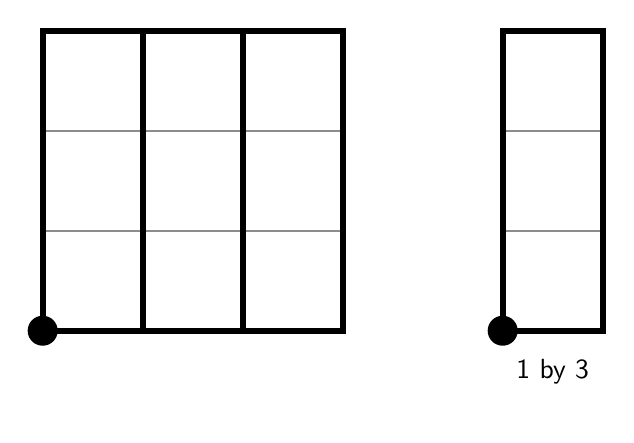
\begin{tikzpicture}[x=1in, y=1in]
\draw[black!45, line width=0.6pt] (0,0) -- (0,1.5);
\draw[black!45, line width=0.6pt] (0.5,0) -- (0.5,1.5);
\draw[black!45, line width=0.6pt] (1,0) -- (1,1.5);
\draw[black!45, line width=0.6pt] (1.5,0) -- (1.5,1.5);
\draw[black!45, line width=0.6pt] (0,0) -- (1.5,0);
\draw[black!45, line width=0.6pt] (0,0.5) -- (1.5,0.5);
\draw[black!45, line width=0.6pt] (0,1) -- (1.5,1);
\draw[black!45, line width=0.6pt] (0,1.5) -- (1.5,1.5);
\draw[line width=2.2pt] (0.5,0) -- (0.5,1.5);
\draw[line width=2.2pt] (1,0) -- (1,1.5);
\draw[line width=2.2pt] (0,0) rectangle (1.5,1.5);
\fill (0,0) circle (0.075);
\draw[black!45, line width=0.6pt] (2.3,0) -- (2.3,1.5);
\draw[black!45, line width=0.6pt] (2.8,0) -- (2.8,1.5);
\draw[black!45, line width=0.6pt] (2.3,0) -- (2.8,0);
\draw[black!45, line width=0.6pt] (2.3,0.5) -- (2.8,0.5);
\draw[black!45, line width=0.6pt] (2.3,1) -- (2.8,1);
\draw[black!45, line width=0.6pt] (2.3,1.5) -- (2.8,1.5);
\draw[line width=2.2pt] (2.3,0) rectangle (2.8,1.5);
\fill (2.3,0) circle (0.075);
\node[anchor=north, inner sep=0pt] at (2.55,-0.14) {\normalsize 1 by 3};
\path (0,-0.42) rectangle (2.8,1.5);
\end{tikzpicture}
\end{center}
\newpage
\prob{8} Is there a table where the ball stops at the corner it started from? Find one, or explain why there is none.
\vspace*{0.05in}
\begin{center}
\begin{tikzpicture}[x=1in, y=1in]
\draw[black!45, line width=0.6pt] (0,0) -- (0,5);
\draw[black!45, line width=0.6pt] (0.5,0) -- (0.5,5);
\draw[black!45, line width=0.6pt] (1,0) -- (1,5);
\draw[black!45, line width=0.6pt] (1.5,0) -- (1.5,5);
\draw[black!45, line width=0.6pt] (2,0) -- (2,5);
\draw[black!45, line width=0.6pt] (2.5,0) -- (2.5,5);
\draw[black!45, line width=0.6pt] (3,0) -- (3,5);
\draw[black!45, line width=0.6pt] (3.5,0) -- (3.5,5);
\draw[black!45, line width=0.6pt] (4,0) -- (4,5);
\draw[black!45, line width=0.6pt] (4.5,0) -- (4.5,5);
\draw[black!45, line width=0.6pt] (5,0) -- (5,5);
\draw[black!45, line width=0.6pt] (5.5,0) -- (5.5,5);
\draw[black!45, line width=0.6pt] (6,0) -- (6,5);
\draw[black!45, line width=0.6pt] (6.5,0) -- (6.5,5);
\draw[black!45, line width=0.6pt] (7,0) -- (7,5);
\draw[black!45, line width=0.6pt] (0,0) -- (7,0);
\draw[black!45, line width=0.6pt] (0,0.5) -- (7,0.5);
\draw[black!45, line width=0.6pt] (0,1) -- (7,1);
\draw[black!45, line width=0.6pt] (0,1.5) -- (7,1.5);
\draw[black!45, line width=0.6pt] (0,2) -- (7,2);
\draw[black!45, line width=0.6pt] (0,2.5) -- (7,2.5);
\draw[black!45, line width=0.6pt] (0,3) -- (7,3);
\draw[black!45, line width=0.6pt] (0,3.5) -- (7,3.5);
\draw[black!45, line width=0.6pt] (0,4) -- (7,4);
\draw[black!45, line width=0.6pt] (0,4.5) -- (7,4.5);
\draw[black!45, line width=0.6pt] (0,5) -- (7,5);
\path (0,-0) rectangle (7,5);
\end{tikzpicture}
\end{center}
\end{document}
